\section*{Problem 1}
\addcontentsline{toc}{section}{Problem 1}

Random vector with the two components uniformely distributed in the unit square [0,1]x[0,1]
Find the probability density function of the product of its components.

\subsection*{Solution}

Let's find the cumulative distribution function of the product of the components of
the random vector:

Let's define the random vector as $X = (A, B)$, where $A$ and $B$ are the components
of the vector.

Then we need to find the probability that $A \cdot B \leq x$.

Reformulating the problem, we need to find the probability that $B \leq \frac{x}{A}$.

Notice that $\frac{x}{A}$ is a hyperbola.

If we transform this problem into a geometric one, we need to find the area below
the hyperbola and inside the unit square, and then divide it by the area of the unit square.

\begin{figure}[h]
    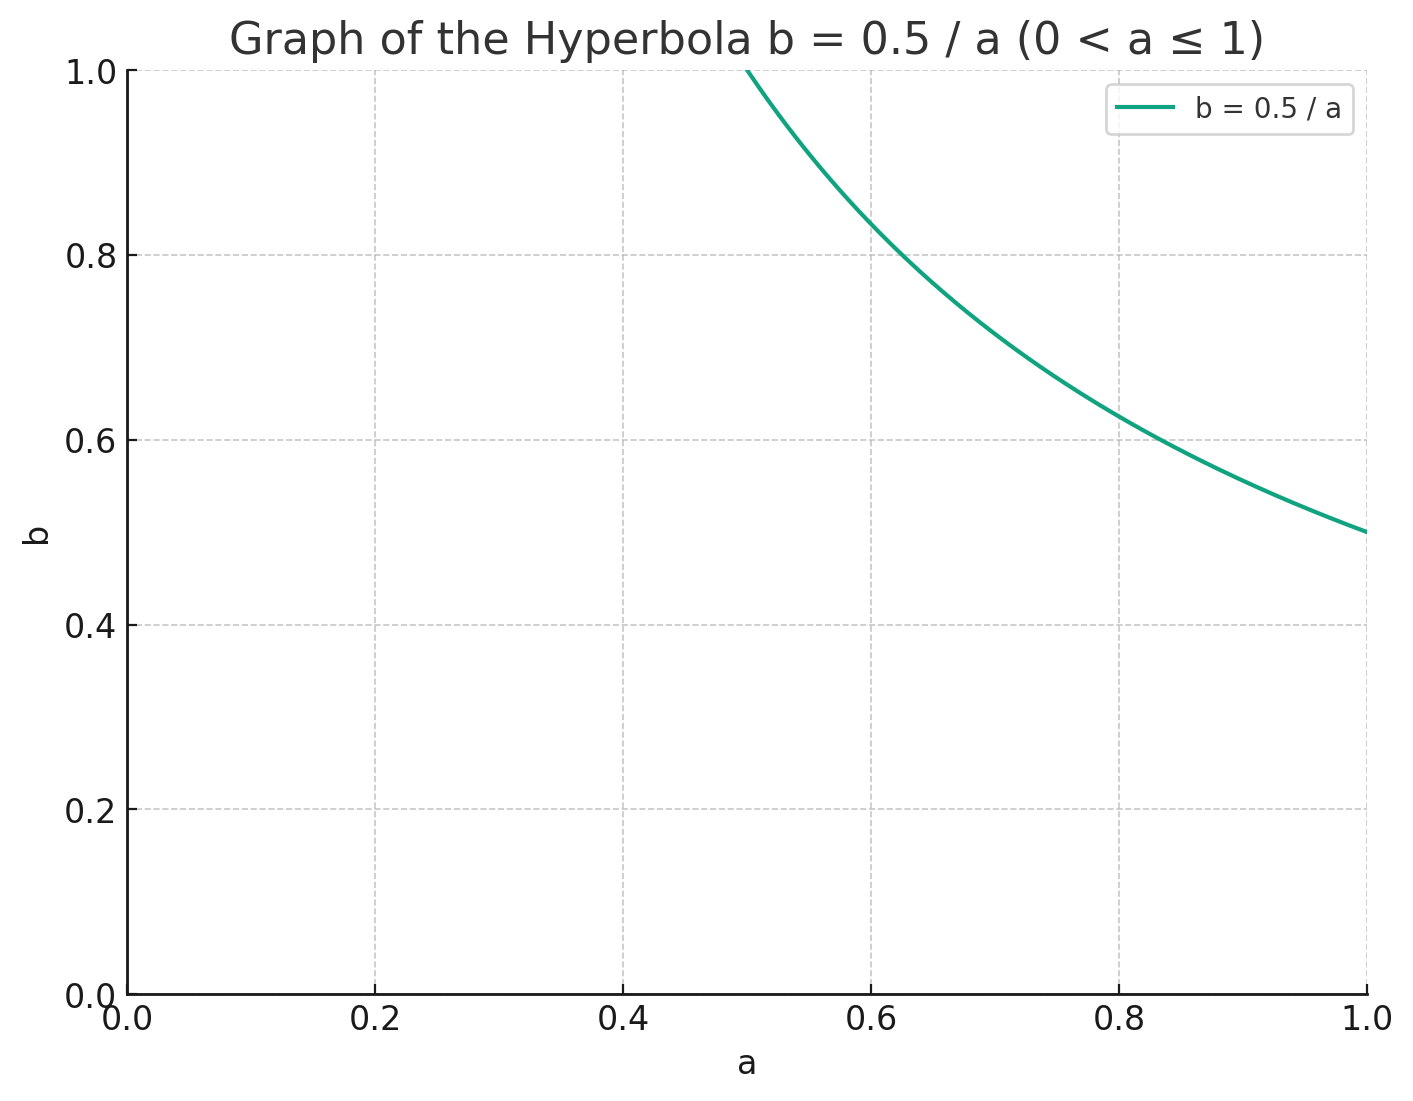
\includegraphics[width=0.8\textwidth]{images/p.jpg}
    \centering
\end{figure}

We can note that the hyperbola intersects the unit square in two points: $(x, 1)$
and $(1, x)$.

So we can decompose this area into a rectangle and an area below the hyperbola.

The area of the rectangle we can calculate finding its width and height, in this
case the width is $x$ and the height is $1$, so the area is $x$.

For the area below the hyperbola we can integrate from range $[x, 1]$ the function
$\frac{x}{A}$ with respect to $A$.

\begin{equation*}
    \int_{x}^{1} \frac{x}{A} dA = x \cdot ln(A) \Big|_{x}^{1} = x \cdot ln(1) - x \cdot ln(x) = -x \cdot ln(x)
\end{equation*}

So the area below the hyperbola is $-x \cdot ln(x)$.

Then the total area is $x - x \cdot ln(x)$.

Now we need to divide it by the area of the unit square, which is $1$,
so the probability is $x - x \cdot ln(x)$.

So we have $3$ cases:

\begin{enumerate}
    \item $x \leq 0$ - the probability is $0$
    \item $0 < x \leq 1$ - the probability is $x - x \cdot ln(x)$
    \item $x > 1$ - the probability is $1$
\end{enumerate}

So the cumulative distribution function is:

\begin{equation*}
    F(x) = \begin{cases}
        0,                 & x \leq 0     \\
        x - x \cdot ln(x), & 0 < x \leq 1 \\
        1,                 & x > 1
    \end{cases}
\end{equation*}

Now we can find the probability density function by differentiating the cumulative
distribution function:

Now let's differentiate when $0 < x \leq 1$:

\begin{equation*}
    f(x) = \frac{d}{dx} (x - x \cdot ln(x)) = 1 - ln(x) - \frac{x}{x} = -ln(x)
\end{equation*}

So the probability density function is:

\begin{equation*}
    f(x) = \begin{cases}
        0,      & x \leq 0,\quad x > 1 \\
        -ln(x), & 0 < x \leq 1
    \end{cases}
\end{equation*}

